
\chapter{Conclusies en perspectieven}
\label{hs:conclusie}

Als slot overlopen we eerst de belangrijkste realisaties van deze masterproef. Daarna overlopen we de hypotheses waarop we aan de hand van de resultaten een antwoord gevonden hebben.

\section{Conclusie}

In deze masterproef werd een client-side routeplanningssysteem opgezet die gebruik maakt van het Linked Connections framework. Er werd een convertor opgezet die een GTFS feed omzet naar connecties. Met deze data werd de basis implementatie van Linked Connections met enkel een tijdsfilter getest. Dit gaf een gemiddelde snelheid van 4.54 seconden per query (\ref{table:gemiddeldesnelheid}). . De onderzoeksvraag van deze masterproef stelt de vraag of dit sneller kan. 

Om een snellere querytijd te bekomen, werden twee andere technieken ontwikkeld. Figuur \ref{ldf-opt} geeft een overzicht van de Linked Data Fragments as met verschillende manieren om routes te plannen. Hierop is te zien hoe de \textit{speed-up} en \textit{heuristische} technieken meer complexiteit van de server eisen om de cli\"ent belasting in te perken.

\begin{figure}[h!]
\centering
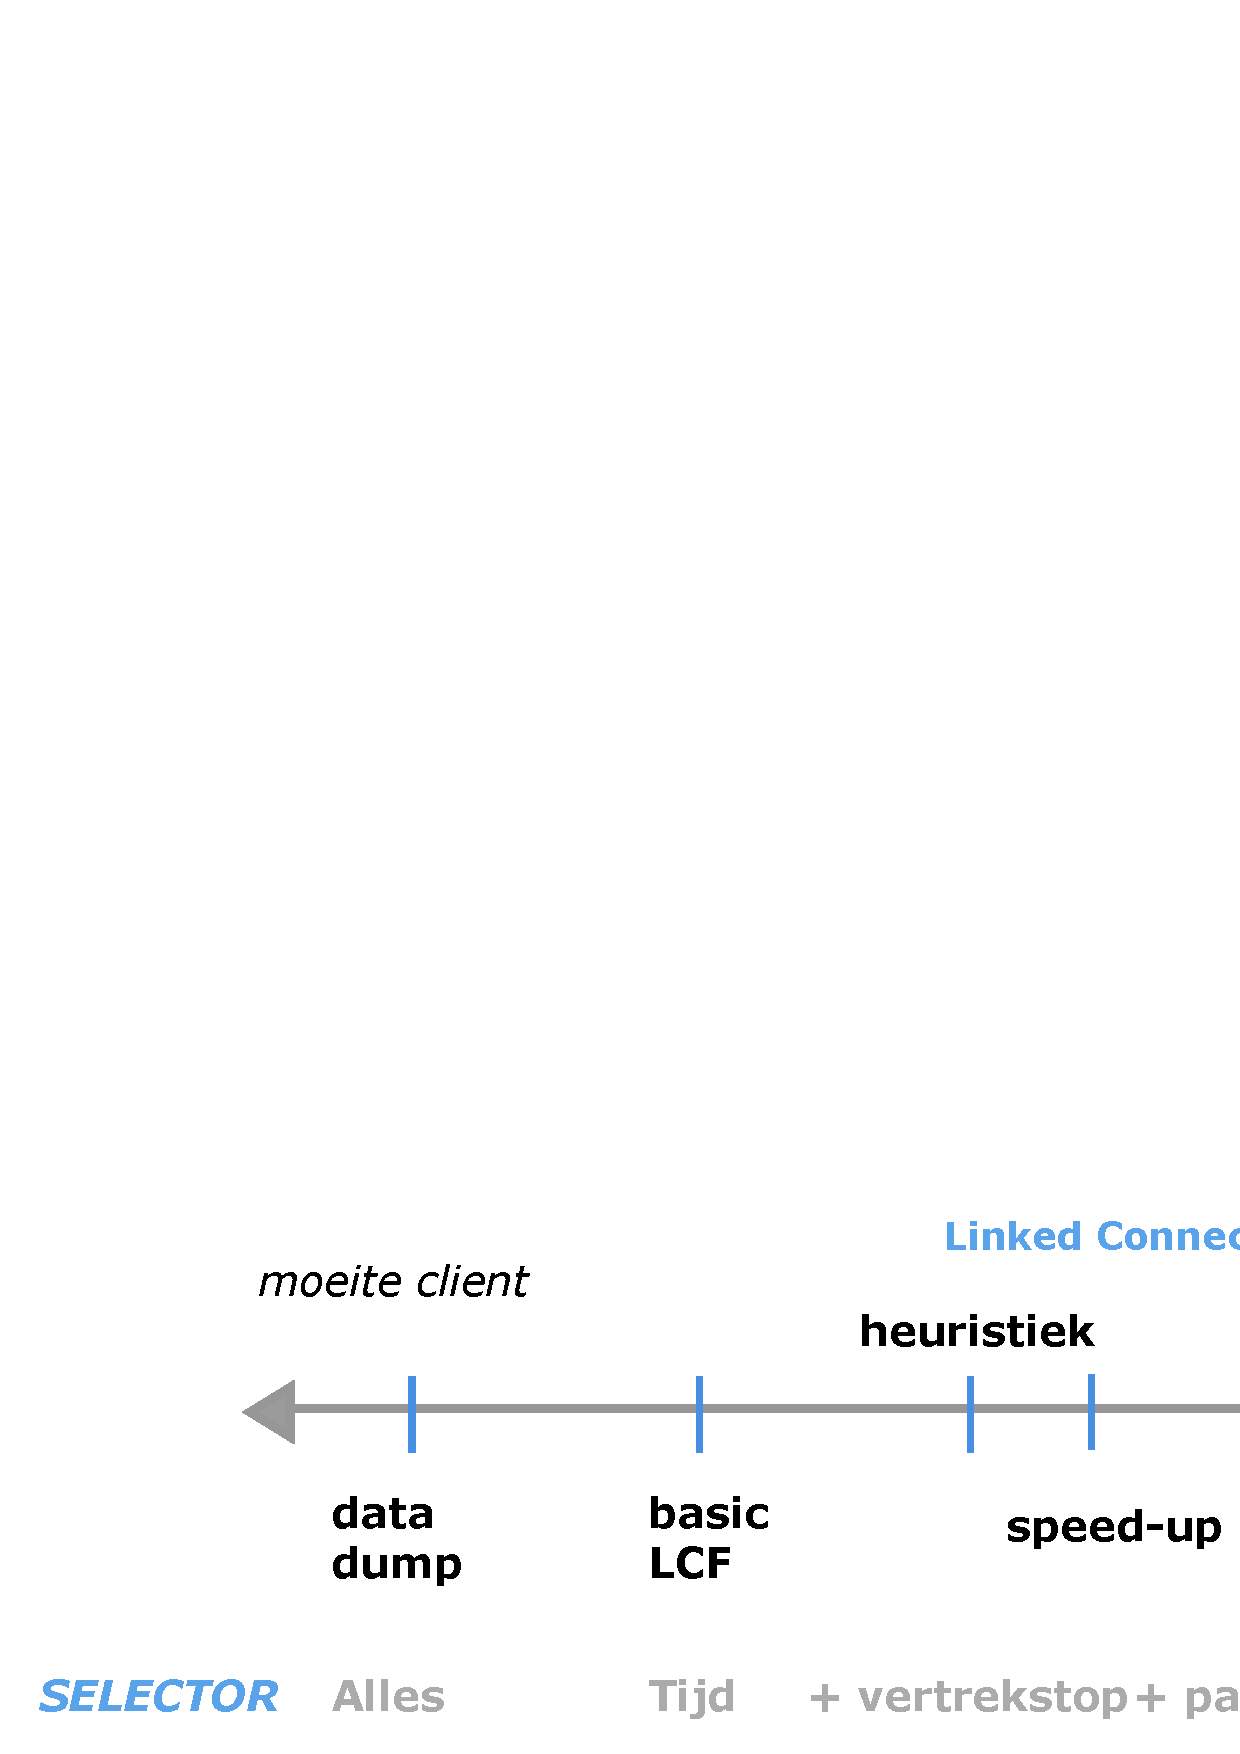
\includegraphics[scale=0.4]{LDF-asFinal.png}
\caption{Linked Data Fragmenten-as met optimalisatietechnieken}
\label{ldf-opt}
\end{figure}

Er werden twee nieuwe termen voor fragmenten ge\"introduceerd: basic Linked Connections Fragments en Neighbouring Linked Connections Fragments (NLCF). Dit laatste fragment maakt gebruik van de tijdsafstand tussen twee stops om connecties te filteren. Zowel de speed-up techniek als de heuristische techniek maken gebruik van deze NLCF's. Uit de resultaten \ref{table:gemiddeldesnelheid} en \ref{tijdmetcachingvolgensaantalstops} kan afgeleid worden dat dit het routeplannen hoogstens dubbel zo snel maakt.

De heuristische methode maakt enkel gebruik van NLCF. De cli\"ent is verantwoordelijk voor het kiezen van een volgende vertrekstop als het resultaat nog niet gevonden is. Om een goede afschatting te maken werd de belangrijkheid van een station gequoteerd aan de hand van het aantal rechtstreeks bereikbare stops. Dit kan makkelijk berekend worden tijdens het genereren van connecties. Bij deze techniek kan echter niet gegarandeerd worden dat de optimale oplossing gevonden wordt. Slechts 78\% van de queries werden optimaal opgelost. Dit kan als een future-work beschouwd worden (zie \ref{max-interval}).

De speed-up techniek garandeert wel dat de optimale oplossing gevonden wordt. De informatie van de eerste NLCF zorgt ervoor dat er minder connecties gescand moeten worden. Deze techniek maakt gebruik van paginering met hypermedia. Deze fragmenten zijn iets kostelijker om te berekenen voor de server. Dit is echter niet erg, omdat de server dynamisch de grootte van de pagina's en fragmenten kan aanpassen afhankelijk van de serverbelasting. Door een grotere fragmentgrootte te kiezen is het mogelijk om de querytijd te verdubbelen ten opzichte van de basis methode (figuren \ref{tijdmetcachingvolgensafstand} en \ref{tijdzondercachingvolgensaantalstops}).

Neighbouring Linked Connections Fragments vergt extra voorbewerking. Het berekenen van de minimale tijdsafstand tussen elke stop vergt weinig extra tijd, omdat dit gebeurt tijdens het genereren van connecties. De extra fase die het minimaal aantal overstappen $K$ berekend is optioneel als extra filter bij de heuristische methode. De heuristische methode geeft van elke stop binnen $K$ een reeks connecties binnen tijdsinterval $T$ terug. Bij grotere netwerken dan de NMBS kan het dus nodig zijn om toch een beperking hierop te stellen. De speed-up techniek beschouwt het aantal overstappen als maximaal om de snelste aankomsttijd te garanderen. Stations die minstens X aantal overstappen nodig hebben, bevinden zich hoogstwaarschijnlijk verder in de tijd waardoor deze connecties toch niet worden teruggeven in het eerste NLCF fragment.

Een andere optimalisatie is het dataverbruik. Door de extra tijdsafstandfilter worden minder nutteloze connecties teruggeven. Dit resulteert in 32\% minder dataverbruik bij de speed-up techniek en 27\% minder bij de heuristische methode. (zie \ref{table:dataverbruik}). In een \textit{real-world} omgeving zal dit waarschijnlijk nog een grotere rol spelen voor de snelheid.

Een laatste aspect die werd gerealiseerd is een \textit{merger} van verschillende connectiestromen. Die zorgt ervoor dat connecties van verschillende Linked Connections servers kunnen opgehaald worden door de cli\"ent. Om intermodaal te kunnen routeplannen moet er een systeem komen die informatie van  stopplaatsen van verschillende feeds semantisch kunnen beschrijven.

We kunnen concluderen dat we geslaagd zijn in op de opzet om client-side routeplannen sneller te maken zonder de garantie te verliezen dat de snelste route gevonden is. Niet alleen snelheid, maar ook dataverbruik is een stuk effici\"enter. Dit gaat ook niet ten koste van extra voorbewerkingstijd.

\chapter{Future work}

\section{Preprocessing}
\label{max-interval}
Tijdens de voorbewerkingsfase wordt voor elke stop de minimale afstand en overstappen tot elke buur bepaald. Een LC server moet connecties binnen een bepaald tijdsinterval teruggeven waarin de snelste route zich bevindt naar elke andere stop. Momenteel werd er verondersteld dat binnen een bepaald tijdsinterval $T$ elke snelste route bepaald kan worden. Een extra feature zou een afschatting zijn van het maximale tijdsinterval waarin connecties moeten teruggegeven worden voor elke stop. Kleine stops hebben bijvoorbeeld een regelmatige verbinding naar een groter station waaruit alle andere stations bereikbaar zijn. Als er binnen het halfuur een connectie bestaat, is het enkel nuttig om connecties binnen het halfuur op te vragen. Voor verafgelegen stations, zoals Basel voor de NBMS, is een groter tijdsinterval nodig.
Door deze informatie kan er met meer zekerheid en effici\"enter enkel de nuttige connecties teruggeven worden.

\section{Multicriteria queries}

Momenteel werd er enkel onderzocht hoe de snelste route gevonden kan worden. Een nieuwe pareto-optimale route zou kunnen beschouwd worden die ook rekening houdt met het maximaal aantal overstappen. CSA zou moeten aangepast worden zodat elke stop meerdere mogelijke oplossingen bijhoudt zodat er niet louter naar de tijd gekeken wordt, maar ook naar de trip. Voor de optimalisatie is dit ook een interessante uitbreiding wegens de manier de data werd voorbewerkt. Elke stop houdt de minimale tijd en het minimaal aantal overstappen naar elke andere stop bij. Er kan zo een extra HTTP parameter toegevoegd worden zodat de cli\"ent kan aanduiden hoeveel overstappen maximaal gemaakt mag worden.

Momenteel wordt er eerst een HTTP request gestuurd om de juiste URL te bekomen van een fragment. Er zou metadata in deze request toegevoegd kunnen worden over de stops die met 0, 1... overstappen bereikbaar zijn. Zo kan de cli\"ent een betere afschatting kunnen doen van het maximaal aantal overstappen.

\section{Intermodaliteit}

Een Linked Connections server is verantwoordelijk voor het aanbieden van connecties van een (of meerdere) provider(s). De cli\"ent moet zelf kunnen beslissen van welke providers data nuttig kan zijn. Een belangrijk aspect hierbij is metadata over stops. Momenteel zijn er geen afspraken over het gebruiken van vaste identifiers voor stops. Enkel zo kan er interoperabiliteit onstaan tussen datasets. Een cli\"ent moet weten of de identifier van de NMBS voor Antwerpen-Centraal dezelfde is als die van de Nederlandse Spoorwegen. Ook moet er geweten zijn welke operatoren en welke soort vervoersmiddelen actief zijn in bepaalde stations of met \textit{footpaths} bereikbaar zijn. 

Een volgende stap zou het combineren zijn van bussen (De Lijn) en treinen (NMBS) die actief zijn binnen dezelfde regio. Er moet gemodelleerd worden wanneer het nuttig is om bepaalde modaliteiten te gebruiken. Het is bijvoorbeeld logisch om bij grote afstanden eerst de trein te nemen en daarna de bus. Desnoods met een bus naar het vertrekstation. Hieruit blijkt dat de vraag naar metadata steeds groter zal zijn. Enkele voorbeelden:

\begin{itemize}
\item faciliteiten zoals rolstoeltoegankelijkheid
\item locatie van perrons
\item mogelijke wandelafstanden
\item gebied waar de publieke vervoersmaatschappij actief is, bijvoorbeeld in GeoJSON-formaat
\item welk soort voertuig
\end{itemize}

Op basis van deze metadata kan een cli\"ent slimme beslissingen nemen om connecties op te halen van de juiste providers. Met behulp van de \textit{merger} die in hoofdstuk \ref{merger} besproken wordt, kunnen de connecties makkelijk gesorteerd samengevoegd worden voor CSA.

\section{Grote netwerken}

Het Connection Scan Algorithm (CSA) is niet schaalbaar voor zeer grote netwerken. Linked Connections werkt snel voor lokale netwerken. Een oplossing hiervoor is  accelerated CSA die we besproken hebben in de literatuurstudie (\ref{acsa}). Deze optimalisatie vereist echter preprocessing. Dit zou toepasbaar kunnen worden binnen Linked Connections door een \textit{accelareted} Linked Connections server te ontwerpen. Wanneer de cli\"ent wil query'en over lange afstanden kan dit eerst hierop gedaan worden. Voor lokale queries kan er dan op de huidige implementatie overgeschakeld worden. 

\subsection{Realtime informatie}

Extra transformer toevoegen die trip van connectie checkt -> update -> hersorteren wel
